\chapter{Planificación}

La planificación de un proyecto llega a ser una de las partes más cruciales del 
desarrollo de este y de su éxito. Es el proceso mediante el cual se definen los 
objetivos, se establecen las tareas y se asignan los recursos necesarios para 
llevar a cabo la creación de un software de manera eficiente y efectiva.

En este capítulo vamos a exponer las distintas metodologías que 
vamos a utilizar tanto para las tareas como para el desarrollo además de dónde se 
puede encontrar el repositorio y las herramientas utilizadas para seguir las 
metodologías.

\section{Metodologías utilizadas}

Decidiendo las distintas metodologías que queremos seguir durante el proyecto, se 
han seleccionado tres metodologías que se llegan a usar en el desarrollo ágil: 
\textbf{Kanban}, \textbf{Desarrollo Dirigido por Pruebas} e \textbf{Integración 
Continua}.

Primero, \textbf{Kanban} \cite{kanban} es una metodología de desarrollo ágil que se 
emplea para visualizar y gestionar el flujo de trabajo de un proyecto, basándose en 
tres tableros: tareas pendientes, en progreso y completadas. Las distintas tareas 
se representan en tarjetas, que vamos moviendo de un tablero a otro según el estado 
de estas.

Nosotros hemos añadido un cuarto tablero, donde pondremos que tareas están 
bloqueadas por otra tarea o proceso. Así, vemos de un vistazo que debemos de 
priorizar para que el proyecto avance (figura \ref{fig:tabla-kanban}).

\begin{figure}[h]
    \centering
    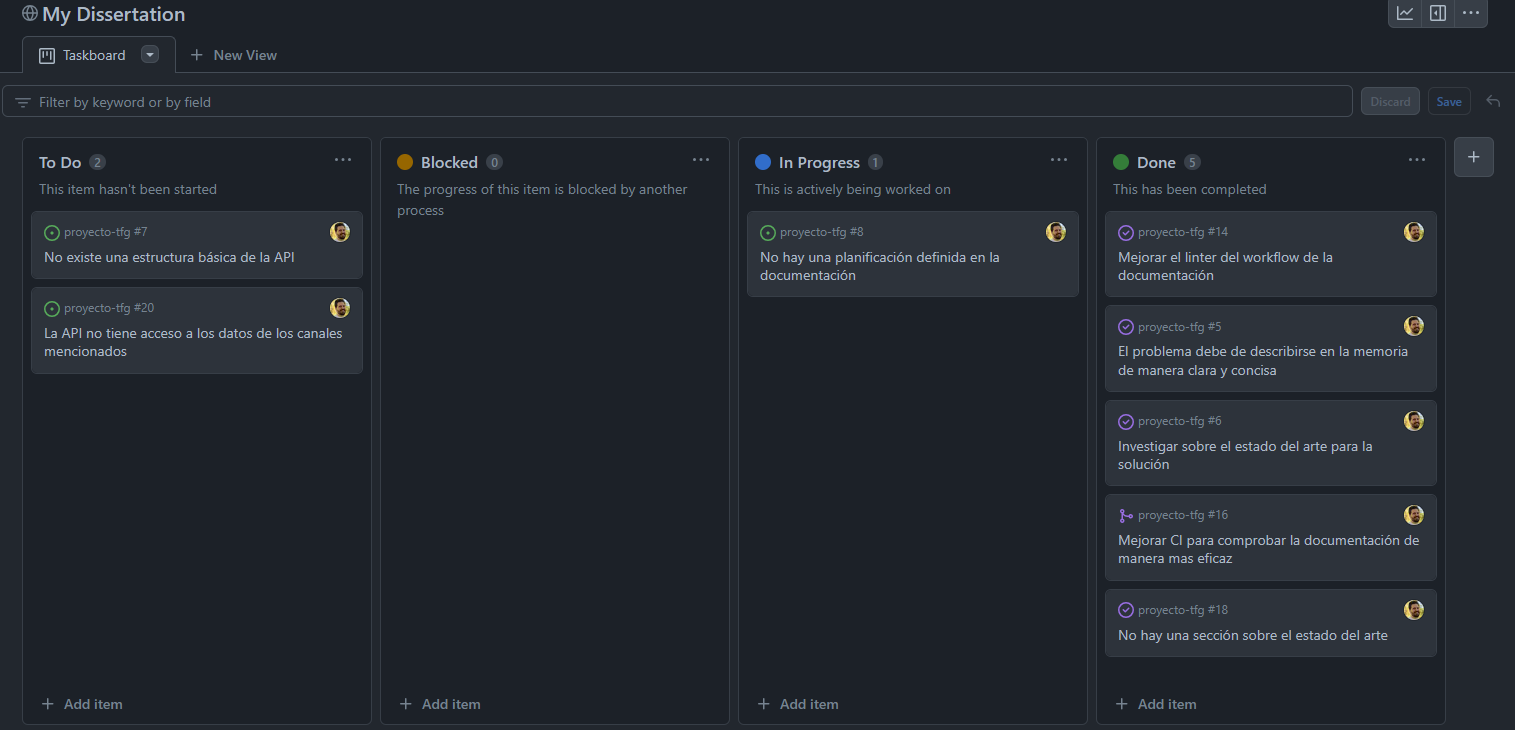
\includegraphics[scale=0.3]{figuras/github-projects-proyecto-tfg.png}
    \caption{Tablas Kanban dentro de GitHub Projects.}
    \label{fig:tabla-kanban}
\end{figure}

El \textbf{Desarrollo Dirigido por Pruebas} (\textbf{TDD}, en inglés \textbf{Test 
Driven Development}) \cite{tdd} es una práctica de desarrollo de software que se 
basa en crear primero las pruebas antes de implementar el código de la 
funcionalidad. Con esto, podemos conseguir tener el código más limpio y que se 
compruebe de manera fácil que el código funciona como indican los requisitos.

Por último, la \textbf{integración continua} (\textbf{CI}, en inglés 
\textbf{Continuous Integration}) \cite{ci} es una metodología de desarrollo de 
software que consiste en integrar los nuevos cambios en el código verificando 
previamente que estos cambios no rompen el código existente. Para llegar a esto, se 
aplicará lo siguiente:

\begin{enumerate}
    \item \textbf{Automatización de pruebas}: Las pruebas (que hemos mencionado 
    anteriormente) serán automatizadas en el flujo de trabajo.
    \item \textbf{Compilación automatizada}: Se compilará el código con los cambios 
    realizados para revisar que no hay problemas durante la compilación.
    \item \textbf{Despliegue automatizado}: Se desplegará el código en un entorno 
    para su acceso en el momento en el que lleguemos al producto mínimo viable.
\end{enumerate}

\section{Seguimiento del desarrollo}

Para el seguimiento del desarrollo del proyecto, hemos decidido usar Git como 
sistema de control de versiones y la plataforma GitHub para alojar el repositorio 
remoto del proyecto.

Lo bueno de GitHub es que, además, nos ofrece más herramientas para seguir las 
distintas metodologías que hemos mencionado anteriormente:

\begin{itemize}
    \item \textbf{GitHub Issues}: Con Issues podemos añadir nuestras tareas para el 
    proyecto para poder saber que hace falta llevar a cabo.
    \item \textbf{GitHub Milestones}: Con Milestones podemos agrupar las tareas que 
    hemos ido creando poco a poco y priorizar lo que se debe de hacer antes, además 
    de tener una ruta clara que debamos de seguir para progresar en el proyecto. 
    Si se quiere ver los distintos Milestones, se puede mediante el siguiente 
    enlace: \url{https://github.com/jero-dev/proyecto-tfg/milestones}
    \item \textbf{GitHub Projects}: Con Projects podemos generar un tablero para 
    seguir la metodología Kanban y comprobar el estado de las tareas o issues que 
    están representadas por las tarjetas (figura \ref{fig:tabla-kanban}). El 
    proyecto se puede encontrar en el siguiente enlace: 
    \url{https://github.com/users/jero-dev/projects/1}
    \item \textbf{GitHub Actions}: Gracias a esta herramienta podemos automatizar 
    tanto la compilación como la ejecución de pruebas cada vez que se añadan 
    cambios. Por tanto, gracias a esto, podemos seguir la metodología de 
    integración continua durante el desarrollo.
\end{itemize}
